\documentclass[conference]{IEEEtran}
\IEEEoverridecommandlockouts

\usepackage{cite}
\usepackage{amsmath,amssymb,amsfonts}
\usepackage{algorithmic}
\usepackage{graphicx}
\usepackage{hyperref}
\usepackage{textcomp}
\usepackage{xcolor}
\def\BibTeX{{\rm B\kern-.05em{\sc i\kern-.025em b}\kern-.08em
    T\kern-.1667em\lower.7ex\hbox{E}\kern-.125emX}}
\begin{document}

\title{The Impact of AI on Education Today\\
%{\footnotesize \textsuperscript{*}Note: Sub-titles are not captured in Xplore and
%should not be used}
%\thanks{Identify applicable funding agency here. If none, delete this.}
}

\author{\IEEEauthorblockN{Azizul Haque Tutul}
\IEEEauthorblockA{\textit{ Department of Computer Science and Engineering} \\
\textit{Dhaka University of Engineering \& Technology, Gazipur}\\
Gazipur, Bangladesh \\
 Email:azizulhaque3695@gmail.com , Student ID : 214052 }
}

\maketitle

\begin{abstract}
Artificial Intelligence (AI) transformed education by enhancing personalized learning, improving administrative efficiency, and providing real-time feedback. It addressed the need for tailored learning experiences and optimized educational outcomes through technology.

AI applications like intelligent tutoring systems, automated grading, and learning analytics showed promise in boosting student engagement and efficiency but faced challenges such as data privacy concerns, biases, and ethical issues.

A proposed model combined AI-driven personalized learning with human oversight, emphasizing ethical deployment, transparency, and inclusivity. This approach used advanced algorithms to deliver tailored learning while protecting student data and ensuring equity.

The results included improved learning outcomes, reduced teacher workload, and better data-driven decisions. AI revolutionized education by supporting human teaching and creating a more personalized and inclusive learning environment
\end{abstract}

\begin{IEEEkeywords}
component, formatting, style, styling, insert
\end{IEEEkeywords}

\section{Introduction}
In recent years, Artificial Intelligence (AI) has gained significant traction in the education sector, transforming traditional teaching and learning methods. The increasing integration of AI into educational practices has been driven by its potential to enhance personalized learning, streamline administrative tasks, and improve overall student engagement and outcomes. Early implementations of AI in education focused on simple computer-assisted instruction, which has since evolved into more complex systems like intelligent tutoring and adaptive learning platforms \cite{r1} \cite{r2} \cite{r5} .AI-powered tools like intelligent tutoring systems and automated grading provided opportunities for real-time feedback, while applications such as text-to-text and text-to-image generators enabled students to explore creative and analytical tasks more effectively \cite{r3} \cite{r6}


Studies also revealed that AI tools contributed to reducing achievement gaps by offering accessible learning resources and adapting to individual learning paces. However, limitations persisted in areas requiring human judgment, such as fostering creativity, empathy, and critical thinking[6,10].However, while the advantages of AI in education are apparent, challenges such as ethical concerns, data privacy issues, and the potential for increased educational inequality must also be addressed \cite{r1} \cite{r4} \cite{r5}


This paper aims to review the current applications of AI in education, explore the benefits and limitations of these technologies, and propose strategies to overcome the associated challenges. By drawing insights from multiple sources, including studies on AI's impact on higher education and its role in enhancing learning outcomes, this review provides a comprehensive understanding of AI's transformative potential in education \cite{r2} \cite{r4} \cite{r5}.Researchers and educators emphasized the need for ethical AI deployment and interdisciplinary collaboration to maximize its potential while addressing these issues \cite{r6} \cite{r10}


As AI applications in education evolved, they reshaped teaching methodologies, opening pathways for educators to complement traditional methods with data-driven insights and adaptive technologies. This progress underscored the importance of informed strategies to ensure AI's responsible and effective use in education \cite{r3} \cite{r6} \cite{r10}



\section{Literature Review}
The use of Artificial Intelligence (AI) in education has been the subject of extensive research, highlighting both its transformative potential and the challenges it poses. The early adoption of AI in education primarily involved computer-assisted learning, which gradually evolved into more sophisticated intelligent tutoring systems (ITS) and adaptive learning platforms\cite{r1} \cite{r2}

Chen et al. (2020) reviewed the integration of AI in education, highlighting its role in automating administrative tasks and personalizing learning experiences. They concluded that AI technologies have significantly improved efficiency and the customization of educational content \cite{r1}.Harry and Sayudin (2023) examined AI's potential to revolutionize education by personalizing learning through machine learning algorithms. Their study underscored the benefits of AI-driven tools like chatbots and automated grading in enhancing educational efficiency and feedback consistency \cite{r2}.Chan and Tsi (2023) explored the role of AI in higher education, particularly its potential to complement or replace human teachers. They suggested that while AI can handle administrative tasks, human teachers' emotional and critical thinking skills remain irreplaceable \cite{r7}


Moreover, AI technologies demonstrated potential in reducing educational disparities. For instance, systems like CENTURY Tech personalized learning by using data-driven insights to cater to individual student requirements. Similarly, tools like Debate Mate used AI to enhance critical skills such as argumentation and collaboration, showcasing AI's ability to foster holistic development \cite{r8} \cite{r10}

Despite these advancements, challenges persisted. Concerns regarding data privacy, algorithmic biases, and ethical considerations in AI implementation were frequently discussed in the literature. Researchers also noted limitations in AI’s ability to support creativity, critical thinking, and social skills, which remain essential for comprehensive education \cite{r3} \cite{r9}

While AI holds promise for reshaping education, its integration requires careful planning. Studies advocated for robust partnerships between AI developers, educators, and researchers to ensure tools meet ethical standards and address the diverse needs of learners. These collaborations are crucial to maximize the benefits of AI while mitigating its risks, paving the way for a more inclusive and effective educational landscape.

\section{Objectives and Outcomes}
\begin{itemize}
    \item  To explore the current applications and theoretical gaps in the integration of AI in education (AIEd).
\end{itemize}

\begin{itemize}
    \item  To establish connections between existing AIEd research and emerging trends in the field.
\end{itemize}

\begin{itemize}
    \item  To provide clear and consistent definitions of AI in education (AIEd) to improve understanding and consistency in future studies
\end{itemize}

\begin{itemize}
    \item  To assess the perceptions and experiences of university students regarding the use of generative AI technologies like ChatGPT in higher education.
\end{itemize}


\begin{itemize}
    \item To highlight the potential benefits, challenges, and ethical considerations associated with the use of AI in education, based on student feedback.
\end{itemize}


\begin{itemize}
    \item  To inform policymakers and educators about the effective implementation of AI technologies to improve teaching, learning, and administrative processes in higher education.
\end{itemize}


\section{Methodologies}

This research employed a qualitative approach to review the role of Artificial Intelligence (AI) in education by analyzing four selected research papers. Each paper was chosen for its relevance to understanding how AI was used in educational settings, the challenges it presented, and its potential for the future.A systematic approach was followed, which involved selecting the documents, analyzing their themes, and combining the findings into a meaningful review.The review aimed to gather insights from different perspectives to provide a comprehensive overview of AI in education.The survey was administered online, consisting of both closed-ended and open-ended questions to gather diverse responses. The questionnaire was developed based on previous studies.Topics included students’knowledge of GenAI technologies, challenges, and the impact of AI on education
\begin{figure}
    \centering
    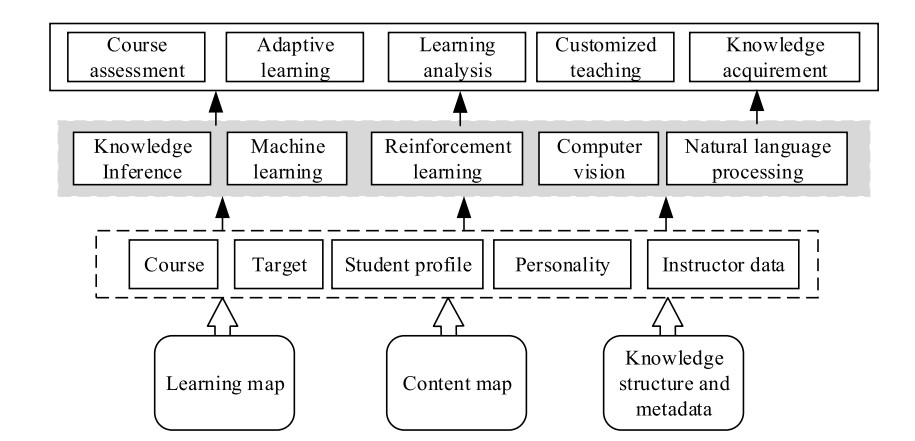
\includegraphics[ width=\linewidth]{picture_1.jpg}
    \caption{Technological structure of AI education \cite{}}
    \label{fig:enter-label}
\end{figure}

\subsection{Document Selection}
Firstly, the articles had to be published in reputable academic journals to ensure the reliability and credibility of the information. Secondly, each article needed to cover a different aspect of AI in education to provide a broad view. For example, Chen et al. (2020) focused on the integration of AI in administrative and instructional tasks, while Harry and Sayudin (2023) emphasized personalized learning and the use of chatbots \cite{r1} \cite{r2}

The research papers were chosen based on their relevance to AI in education. The first paper explored student perceptions of generative AI, focusing on benefits like personalized learning and challenges such as data privacy and biases \cite{r3} The sixth paper examined the integration of learning sciences with AI to design effective educational technologies, highlighting the importance of interdisciplinary approaches \cite{r6} . The tenth paper provided real-world examples of AI applications in education, such as tutoring systems and automated grading, while discussing its potential for scalability and accessibility [10]. Selwyn (2022) discussed the ethical concerns and limitations of AI in education, and Chan and Tsi (2023) explored the potential for AI to either replace or assist human teachers\cite{r8} \cite{r5}

\subsection{Data Collection Process}
The data collection process involved a detailed reading and analysis of each selected article. Key themes and findings were identified and categorized under headings such as AI applications, benefits, challenges, and future implications. For instance, while Chen et al. (2020) highlighted the efficiency gains from AI-driven administrative tasks, Selwyn (2022) raised concerns about data privacy and potential biases \cite{r1} \cite{r4}

To ensure reliability, insights from all three documents were compared. This process identified common trends, such as the potential for AI to enhance equity in education, and disparities, like the varying levels of evidence supporting AI’s scalability. Cross-referencing these findings ensured a balanced perspective

\subsection{Analysis of Data}

The analysis was conducted by comparing the key themes across the four articles. This comparative analysis helped to identify common trends, such as the emphasis on personalized learning and the use of AI for administrative efficiency. It also revealed differences in focus, with some articles highlighting the benefits of AI in education and others emphasizing the challenges and ethical concerns. For example, Harry and Sayudin (2023) discussed the efficiency of automated grading, while Chan and Tsi (2023) explored the irreplaceable human qualities of teachers that AI could not replicate

\begin{figure} [h]
    \centering
    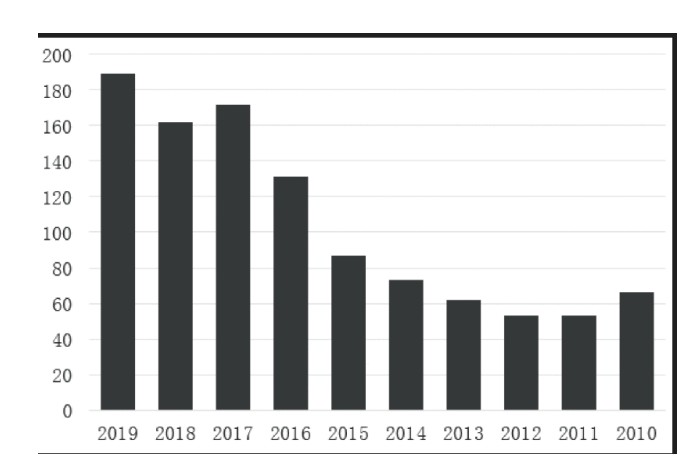
\includegraphics[width=\linewidth]{picture_2.jpg}
    \caption{Papers in Web of Science and Google Scholar in the last ten year with key words “AI” and “Education”[1]}
    \label{fig:enter-label}
\end{figure}

\subsection{Thematic Analysis}
The analysis aimed to identify recurring themes related to AI’s role in education. A detailed reading of each document was conducted to extract information about:

\begin{itemize}
    \item Applications: AI tools and their uses in personalized learning, grading, and student engagement
\end{itemize}

\begin{itemize}
    \item Benefits: Enhancements in teaching efficiency, equity, and learner outcomes
\end{itemize}

\begin{itemize}
    \item Challenges: Ethical concerns, privacy risks, and limitations in creativity and critical thinking.
\end{itemize}

\begin{itemize}
    \item Recommendations: Proposed strategies for ethical AI integration and interdisciplinary collaboration
\end{itemize}

\subsection{Benefits for Students and Teachers}
This methodology helped identify how AI could assist both students and teachers in educational settings. For students, the findings showed that AI could personalize learning, adapt to individual learning paces, and provide immediate feedback, making learning more accessible and tailored to individual needs. Students who face difficulties in specific areas could use AI to get extra support and improve their skills.

For Teachers AI reduced the time spent on repetitive tasks, like grading papers or tracking attendance, allowing teachers to focus on teaching and mentoring students. AI-generated reports gave teachers a clear view of student performance, helping them design better lessons and address individual challenges. By understanding these benefits, educators could better integrate AI tools into their classrooms to improve the overall educational process

\section{Results}
The first paper by Chen et al. (2020) showed that AI had been successfully used to automate administrative tasks in schools and universities. Tasks like grading assignments and tracking student performance were made more efficient, which allowed teachers to spend more time on teaching \cite{r1}

AI also made education more accessible by providing real-time feedback and allowing students to learn at their own pace. For students with disabilities or those who could not attend regular classes, AI created opportunities to learn through virtual classrooms and adaptive technologies \cite{r10}

AI in education enables personalized learning, adjusting to each student’s unique
needs, strengths, and interests. It uses machine learning to analyze students’ behavior,
preferences, and achievements, tailoring their learning experience. For example, AI can
recommend resources, suggest improvements, and adjust task difficulty. The key benefits include supporting struggling students and challenging advanced ones. Personalized
learning boosts engagement, motivation, and academic performance, leading to better retention

\begin{figure}[h]
    \centering
    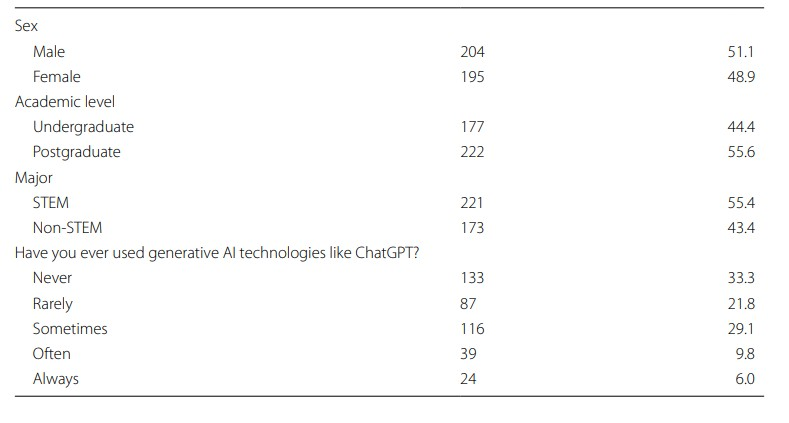
\includegraphics[height= 7cm, width=\linewidth]{picture_3.jpg}
    \caption{ Demographic Information [3]}
    \label{fig:enter-label}
\end{figure}

AI tools offered students personalized learning experiences by tailoring lessons to their individual needs. For example, intelligent tutoring systems helped students improve their understanding of complex subjects by providing targeted support. Tools like ChatGPT assisted with brainstorming and writing, especially for non-native English speakers \cite{r3} \cite{r9}

Selwyn (2022) highlighted the challenges of using AI in education, especially around issues of data privacy and algorithmic bias. This paper stressed the importance of ethical considerations when implementing AI in classrooms to avoid unfair treatment of students \cite{r4}


\section{Discussion}
The results showed that AI had the potential to greatly improve the educational experience for students by offering personalized learning and efficient administrative support. For example, AI systems could quickly grade tests and provide feedback, which saved teachers time and helped students learn more effectively. However, the discussion also raised concerns about the ethical use of AI, especially regarding the privacy of student data and the fairness of AI decisions.

One of the key discussions was about the balance between AI and human teachers. The findings from Chan and Tsi (2023) made it clear that while . Teachers brought unique qualities like empathy and the ability to inspire students, which AI could not replicate. This suggested that the best approach was to use AI as a tool to support teachers rather than as a substitute.

Another key point was that AI should complement, not replace, teachers. While AI could handle repetitive tasks and provide personalized lessons, it could not build relationships, motivate students, or teach soft skills. Teachers remained essential for guiding students and creating a supportive learning environment


AI can also analyze past performance, identify weaknesses, and adapt the pace of instruction, ensuring a more effective learning experience.

\section{challenge }

One of the biggest challenges in using Artificial Intelligence (AI) in education was protecting student data. AI systems collected large amounts of personal information, which raised concerns about how this data was stored and used. Misuse of this information could lead to breaches of privacy \cite{r3} \cite{r8}

Over-reliance on AI tools might discourage students and teachers from developing critical thinking and problem-solving skills. There was also a risk that some students, especially in underprivileged areas, might not have access to the technology needed to use AI systems \cite{r10}

The review revealed several challenges in integrating AI into education, primarily data privacy and security. AI systems need vast student data, posing risks of misuse. Selwyn (2022) stressed the need for robust data protection to keep student information secure \cite{r4}

Ethical considerations were also highlighted, with Chan and Tsi (2023) emphasizing that while AI could assist teachers, it should not replace them, as human interaction is essential for critical thinking and emotional development in students \cite{r10}

\section{Future Work}

Future research should focus on creating ethical AI systems that prioritize data privacy and security. Clear policies and regulations are needed to ensure AI tools handle sensitive student information responsibly \cite{r8} Efforts should be made to reduce biases in AI algorithms and improve their accuracy. This could be achieved by using more diverse datasets and involving educators in the development process to make sure AI tools address real-world needs \cite{r3} \cite{r6} 

AI should be designed to work alongside teachers rather than replace them. Future work could explore ways to enhance collaboration between AI tools and human educators, allowing teachers to focus on building relationships and fostering creativity in the classroom\cite{r6} \cite{r10} 

Additionally, there is a need for continuous professional development for educators. Teachers should be trained to effectively use AI tools in their teaching practices, which will require ongoing support and learning opportunities. This will ensure that educators are equipped to maximize the benefits of AI while mitigating any challenges.

Finally, addressing policy and ethical frameworks will be crucial for the future of AI in education. Governments and educational institutions should work together to develop guidelines that ensure the ethical use of AI, protecting students' rights and promoting fairness across educational systems

\section{conclusion}
The review of the selected papers showed that Artificial Intelligence (AI) had a significant impact on education by enhancing personalized learning and reducing teachers' administrative workload.
However, it also highlighted several challenges, including data privacy concerns, potential biases in AI algorithms, and ethical considerations. The findings emphasized that while AI could greatly assist in educational processes, it could not replace the human elements that teachers bring, such as empathy, creativity, and critical thinking.

Despite these challenges, AI showed great promise in enhancing education when used as a supportive tool alongside human expertise. Future research and innovation could focus on improving fairness, expanding accessibility, and understanding the long-term impacts of AI in education.Future efforts needed to focus on addressing these challenges and ensuring that AI was used as a supportive tool to improve the overall educational experience.

\bibliographystyle{ieeetr}
\bibliography{ref.bib}

\end{document}